\documentclass[journal,a4paper]{Imperial_lab_report}
\usepackage[T1]{fontenc}
\usepackage{amsmath,graphicx,cite}
\usepackage[hidelinks]{hyperref}
\graphicspath{{images/}}
\hyphenation{radio-activity photo-diode}
\begin{document}
\title{Investigating Deviations from the Inverse-Square Law in Beta Radiation Measurements}
\author{Qiyue Chen}
\markboth{Q. Chen}{Beta-Counting Distance Dependence}
\maketitle
\begin{abstract}
We investigate departures from inverse-square counting in a strontium-90 distance scan using geometry, timing and particle-transport models. The last three readings at each of 32 separations give a raw count-rate product that rises from $1.83$ to $13.33$ and falls to $9.83\,\mathrm{m^2s^{-1}}$. An estimated 2~$\mu$s recovery scale implies a 3.8\% correction at the closest position under a non-paralysable model. For an assumed 21~mm distance offset, the exact square-detector correction is 2.5\% there, whereas changing the offset substantially alters the prediction. A matched air/vacuum Geant4 comparison predicts decreasing beta-detection probability in air. The tested models do not uniquely explain the scan; unknown geometry and detector response limit both causal attribution and an absolute activity estimate.
\end{abstract}
\section{Question and measurement}
For an isotropic point emitter and a small detector of area $S$, $c\simeq K/r^2$, so $cr^2$ is constant if detection efficiency and transmission are independent of distance \cite{script}. We ask how much the observed departure can be explained by effective separation, finite geometry, counting losses and beta transport.

A sealed $^{90}$Sr source and an S3590-09 silicon detector (nominal $10\times10\,\mathrm{mm^2}$ active area \cite{sensor}) faced each other on a rail. The recorded distance $d$ was the moving scale reading minus the fixed base width of 50~mm. Source and detector were aligned visually. The last three count--time records at each of 32 positions were retained, as specified before this analysis; all 141 original observations remain in the data archive. Selected exposures were 5--65~s each. The recorded distance is not necessarily the active-plane separation, modelled as $r=d+\delta$; $\delta=16$--25~mm is a sensitivity range, not a measured confidence interval.

For total selected counts $N$ and time $t$, $c=N/t$ and $u=cd^2$. We use the Book2 worksheet's Poisson and reading-error expression,
\begin{equation}
 s_u=u\sqrt{1/N+(2s_d/d)^2},\qquad s_d=0.5\ {\rm mm}.
 \label{eq:unc}
\end{equation}
Book2 treats 0.5~mm directly as a standard uncertainty. This excludes common zero-offset, alignment and response errors; its Poisson assumption is examined below.
\begin{figure}[!t]
\centering
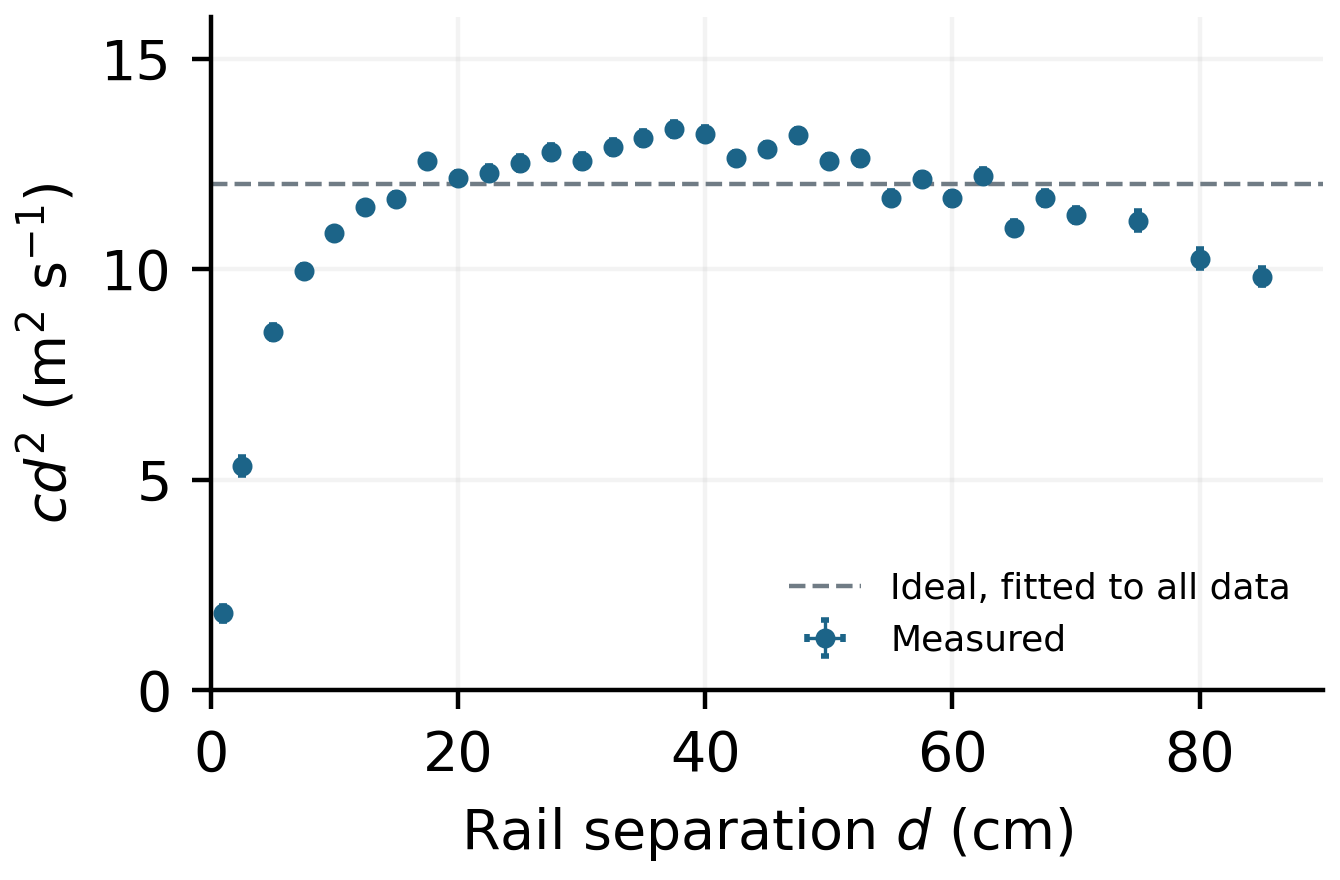
\includegraphics[width=\columnwidth]{report_data.png}
\caption{Raw $cd^2$ with horizontal rail-reading and vertical Eq.~(\ref{eq:unc}) standard errors. The dashed ideal line is fitted to all 32 count rates, not chosen as a plateau. Its poor conditional fit does not by itself identify a cause.}
\label{fig:data}
\end{figure}

\section{Models and analysis}
For a point emitter on the normal axis of a square detector with half-width $a=5$~mm, the exact solid angle is
\begin{equation}
 \Omega(r)=4\tan^{-1}\!\frac{a^2}{r\sqrt{r^2+2a^2}}.
 \label{eq:omega}
\end{equation}
The finite-area factor relative to $S/r^2$ is $F=\Omega/(S/r^2)$. A geometry-only importance-sampled Monte Carlo integrates isotropic emission over an illustrative 22~mm-diameter circular source and the square surface. Eight independently scrambled batches of $2^{15}$ samples estimate numerical error; source radius and absence of aperture shading are assumptions.

The recent time-interval histogram has 500 bins over a user-confirmed 31.25~$\mu$s. A descriptive Gaussian recovery-delay plus exponential waiting-time fit gives $\tau_{\rm eff}=2.00\,\mu$s, conditional on treating the final bin as overflow. The CSV does not independently document that convention, and $\tau_{\rm eff}$ is not a calibrated hard dead time. We test both non-paralysable and paralysable throughput models \cite{pomme}; neither is established as the actual response.

Matched Geant4 air/vacuum simulations use the same assumed 21~mm offset, 1/3~mm transverse shifts, 22~mm emitting disc, 11~mm aperture and 10~keV silicon-deposition threshold \cite{geant,livermore}. These are model inputs, not calibrated values. The assumed Sr/Y beta endpoints are approximately 0.55/2.3 MeV \cite{iaea}. $T=p_{\rm air}/p_{\rm vac}$ includes energy loss, scattering and threshold response. Eight air batches and 12 vacuum batches provide Monte Carlo covariance at eight simulated distances. Source histories are not multiplied by the number of distances when quoting independent statistics.

\begin{figure}[!t]
\centering
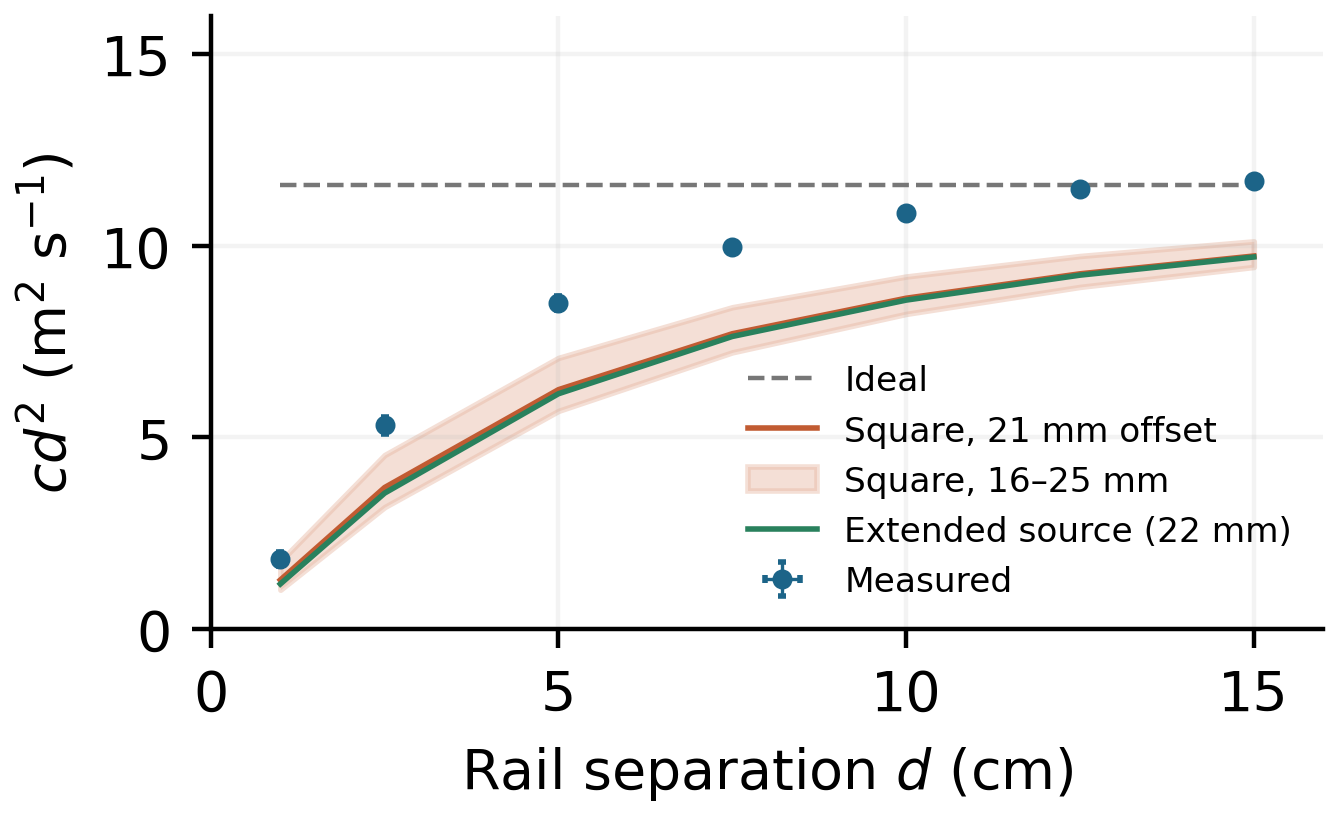
\includegraphics[width=\columnwidth]{report_geometry.png}
\caption{Near-field geometry-only predictions: ideal, on-axis square and illustrative extended source. Each amplitude uses only the same 30, 50 and 85~cm points; near points are not used for scaling. The shaded 16--25~mm offset envelope is a scenario range, not a confidence band. Neither aperture nor air transport is included.}
\label{fig:geo}
\end{figure}

\section{Results and interpretation}
The raw product rises from $1.828\pm0.183$ at 1~cm to 13.33 at 37.5~cm, and falls to $9.826\pm0.208\,\mathrm{m^2s^{-1}}$ at 85~cm (Fig.~\ref{fig:data}). From 30 to 85~cm it falls by 21.8\%. For the all-distance ideal fit, $\chi^2=2002$ for 31 degrees of freedom under a log-rate Gaussian approximation combining Poisson error and $s_d$ once. Its nominal $p<10^{-300}$ is conditional on the assumed independent errors, not a full systematic test.

\emph{Near field.} At $d=10$~mm, $\delta=21$~mm implies $r=31$~mm. Equation~(\ref{eq:omega}) gives $F=0.975$: the point-source finite-square effect is 2.5\%, not the whole near-field departure. Varying $\delta$ from 16 to 25~mm changes the nearest point-source geometric acceptance from 0.01135 to 0.00637 per isotropically emitted beta. An assumed 22~mm source reduces it to 0.00742 at $r=31$~mm, versus 0.00807 for a point source. These examples omit source apertures and material (Fig.~\ref{fig:geo}).

At the nearest measured rate, taking $\tau_{\rm eff}$ as a hard response time increases the inferred rate by 3.79\% in the non-paralysable model or 3.87\% in the paralysable model. These are sensitivity estimates, not measured losses. A free-offset $K/(d+\delta)^2$ fit gives $\delta_{\rm fit}=11.4$~mm but $\chi^2/\nu=981/30$ under the same conditional errors. The fitted parameter is model-dependent, not an independent measurement of the hardware.

\emph{Far field and limitations.} Geant4 gives $T(30\,\mathrm{cm})=0.778\pm0.047$ and $T(85\,\mathrm{cm})=0.423\pm0.063$ (Monte Carlo errors only). Transport can therefore change the distance response, but the input spectrum, encapsulation and detector threshold are unvalidated. The older Task16 record gives 8 background counts in 60~s; at 85~cm this contributes $0.096\,\mathrm{m^2s^{-1}}$ to raw $cd^2$ and acts upward. It is not established as the background during the later scan.

A hybrid square-geometry model multiplied by the simulated $T$ and a working 2~$\mu$s loss model gives nominal $\chi^2/\nu=25.9/7$ at the eight simulated distances, using their correlated Monte Carlo uncertainty and fitting one scale. This mixed model and its inputs were considered after observing data; it does not validate the apparatus. Twelve explicit first/return pairs yield $Q=54.0$ for 12 degrees of freedom ($p=2.7\times10^{-7}$ for stationary independent Poisson counts), indicating additional variation. It does not determine its cause. Consequently the nominal model significances above omit important uncertainties; AIC/BIC ranking is not warranted.

\section{Activity and conclusion}
If secular equilibrium gives approximately two beta emissions per $^{90}$Sr decay and a constant average detection efficiency $\bar\epsilon$, the ideal relation is $K=A_{\rm Sr}(2\bar\epsilon)S/(4\pi)$. The provisional $\delta=21$~mm point fit gives the formal product $A_{\rm Sr}\bar\epsilon\simeq0.90$~MBq; offset scenarios give 0.86--0.93~MBq. The underlying fits are poor and transmission and efficiency are not calibrated, so neither an absolute activity nor a defensible total uncertainty follows. The source reference activity and date require verification.

The distance reference, transport and detector response can all alter $cd^2$; their separate contributions remain underdetermined. Measuring the active-plane offset and aperture, repeating fixed-distance alignment scans, and independently testing count-rate linearity would most improve the model.
\begin{thebibliography}{6}
\bibitem{script} Imperial College London, \emph{Radioactivity}, Year 2 laboratory script, 2026, Tasks 14--17.
\bibitem{sensor} Hamamatsu Photonics, \emph{Si PIN Photodiodes: S3590 Series}, KPIN1052E11, 2020.
\bibitem{pomme} S.~Pomm\'e, J.~Keightley and R.~Fitzgerald, ``Uncertainty of nuclear counting,'' \emph{Metrologia}, vol.~52, S3, 2015, doi: \href{https://doi.org/10.1088/0026-1394/52/3/S3}{10.1088/0026-1394/52/3/S3}.
\bibitem{geant} S.~Agostinelli \emph{et al.}, ``Geant4---a simulation toolkit,'' \emph{Nucl. Instrum. Methods A}, vol.~506, pp.~250--303, 2003, doi: \href{https://doi.org/10.1016/S0168-9002(03)01368-8}{10.1016/S0168-9002(03)01368-8}.
\bibitem{iaea} IAEA, \href{https://nucleus.iaea.org/sites/fcris/SitePages/Pestiside-Attributes/STRON.htm}{``Strontium-90, nuclide record}.
\bibitem{livermore} Geant4 Collaboration, \href{https://geant4.web.cern.ch/documentation/dev/plg_html/PhysicsListGuide/electromagnetic/Liv.html}{``EM Liv,'' \emph{Physics List Guide}}, v.~11.4.
\end{thebibliography}
\end{document}
